%%%%%%%%%%%%%%%%%%%%%%%%%%%%%%%%%%%%%%%%%%%%%%%%%%%%%%%%%%%%%%%%%%%%%%%
% Universidade Federal de Santa Catarina             
% Biblioteca Universitária                     
%----------------------------------------------------------------------
% Exemplo de utilização da documentclass ufscThesis
%----------------------------------------------------------------------                                                           
% (c)2013 Roberto Simoni (roberto.emc@gmail.com)
%         Carlos R Rocha (cticarlo@gmail.com)
%         Rafael M Casali (rafaelmcasali@yahoo.com.br)
%%%%%%%%%%%%%%%%%%%%%%%%%%%%%%%%%%%%%%%%%%%%%%%%%%%%%%%%%%%%%%%%%%%%%%%
\documentclass{ufscThesis} % Definicao do documentclass ufscThesis	

%----------------------------------------------------------------------
% Pacotes usados especificamente neste documento
\usepackage{graphicx} % Possibilita o uso de figuras e gráficos
\usepackage{color}    % Possibilita o uso de cores no documento
\usepackage{pdfpages} % Possibilita a inclusão da ficha catalográfica
\usepackage{listings}
\usepackage{float}
\usepackage{fancyhdr}
\usepackage{subcaption}


%----------------------------------------------------------------------
% Comandos criados pelo usuário
\newcommand{\afazer}[1]{{\color{red}{#1}}} % Para destacar uma parte a ser trabalhada
\newcommand{\ABNTbibliographyname}{REFERÊNCIAS} % Necessário para abnTeX 0.8.2


%----------------------------------------------------------------------
% Identificadores do trabalho
% Usados para preencher os elementos pré-textuais
\instituicao[a]{Universidade Federal de Santa Catarina} % Opcional
\departamento[a]{Engenharia Mecânica}
\curso[o]{Programa de Pós-Graduação}
\documento[o]{Dissertação} % [o] para dissertação [a] para tese
\titulo{Radiação normal de dutos com escoamento subsônico e diferentes condições de contorno}
\subtitulo{análise numérico-experimental} % Opcional
\autor{José Pedro de Santana Neto}
\grau{Mestre em Engenharia Mecânica}
\local{Florianópolis} % Opcional (Florianópolis é o padrão)
\data{15}{Junho}{2016}
\orientador[Orientador]{Andrey Ricardo da Silva, Ph.D.}
%\coorientador[Coorientador]{Henrique Simas, Dr. Eng.}
\coordenador[Coordenador]{Armando Albertazzi Gonçalves Júnior, Dr. Eng.}

\numerodemembrosnabanca{3} % Isso decide se haverá uma folha adicional
\orientadornabanca{sim} % Se faz parte da banca definir como sim
\coorientadornabanca{nao} % Se faz parte da banca definir como sim
\bancaMembroA{Primeiro membro\\Universidade ...} %Nome do presidente da banca
\bancaMembroB{Segundo membro\\Universidade ...}      % Nome do membro da Banca
\bancaMembroC{Terceiro membro\\Universidade ...}     % Nome do membro da Banca
\bancaMembroD{Quarto membro\\Universidade ...}       % Nome do membro da Banca
%\bancaMembroE{Quinto membro\\Universidade ...}       % Nome do membro da Banca
%\bancaMembroF{Sexto membro\\Universidade ...}        % Nome do membro da Banca
%\bancaMembroG{Sétimo membro\\Universidade ...}       % Nome do membro da Banca

\dedicatoria{Este trabalho é dedicado aos meus colegas de classe e aos meus queridos pais.}

\agradecimento{Inserir os agradecimentos aos colaboradores à execução do trabalho.}

\epigrafe{Texto da Epígrafe. Citação relativa ao tema do trabalho. É opcional. A epígrafe pode também aparecer na abertura de cada seção ou capítulo.}
{(Autor da epígrafe, ano)}

\textoResumo {O texto do resumo deve ser digitado, em um único bloco, sem espaço de parágrafo. O resumo deve ser significativo, composto de uma sequência de frases concisas, afirmativas e não de uma enumeração de tópicos. Não deve conter citações. Deve usar o verbo na voz passiva. Abaixo do resumo, deve-se informar as palavras-chave (palavras ou expressões significativas retiradas do texto) ou, termos retirados de thesaurus da área.}
\palavrasChave {Palavra-chave 1. Palavra-chave 2.  Palavra-chave 3. }
 
\textAbstract {Resumo traduzido para outros idiomas, neste caso, inglês. Segue o formato do resumo feito na língua vernácula. As palavras-chave traduzidas, versão em língua estrangeira, são colocadas abaixo do texto precedidas pela expressão ``Keywords'', separadas por ponto.}
\keywords {Keyword 1. Keyword 2. Keyword 3.}

%----------------------------------------------------------------------
% Início do documento                                
\usepackage{comandos}

\begin{document}
%--------------------------------------------------------
% Elementos pré-textuais
\capa  
%\folhaderosto[comficha] % Se nao quiser imprimir a ficha, é só não usar o parâmetro
%\folhaaprovacao
%\paginadedicatoria
%\paginaagradecimento
%\paginaepigrafe
%\paginaresumo
%\paginaabstract
%\pretextuais % Substitui todos os elementos pre-textuais acima
%\listadefiguras % as listas dependem da necessidade do usuário
%\listadetabelas 
%\listadeabreviaturas
%\listadesimbolos
%%%%%%
%\f
\sumario
%--------------------------------------------------------
% Elementos textuais
%%%%%%%%%%%%%%%%%%%%%%%%%%%%%%%%%%%%%%%%%%%%%%%%%%%%%%%%%%%%%%%%%%%%%%%%

\chapter{Introdução}
\label{chapter:introdcao}

A propagação e irradiação de modos normais (ondas planas) é um problema clássico em acústica e continua tendo importância significativa mediante ao advento de novas tecnologias relacionadas a sistemas de exaustão, distribuição de massa, motores aeronáuticos, instrumentos musicais e assim por diante.

Em geral, pode-se utilizar três parâmetros para caracterizar o fenômeno abordado:

\begin{itemize}
    \item a magnitude do coeficiente de reflexão $\|R\|$, razão entre as componentes refletida e incidente da onda no duto, a qual é dada por
    \begin{equation}
        R_{r} =\frac{Z_{r} - Z_{0}}{Z_{r} + Z_{0}},
        \label{eq:R}
    \end{equation}
    sendo $Z_{r}$ a impedância de radiação e $Z_{0}$ a impedância característica do meio;
    
    \item coeficiente de correção da terminação normalizado pelo raio do duto $l/a$ em que $a$ é o raio do duto. Tal parâmetro representa o comprimento acústico efetivo do duto. Em outras palavras, o fator $l$ é a quantidade adicional medida a partir da abertura do duto a qual deve propagar a onda incidente antes de ser refletida para o interior do duto com fase invertida. Tal coeficiente de correção da terminação $l$ é dado por
    \begin{equation}
        l = \frac{1}{k} \arctan\!\left(\frac{Z_{r}}{Z_{0} \, \mathrm{i}}\right)
        \label{eq:l}
    \end{equation}
    sendo $k$ o número de onda;
    
    \item diretividade $G(f,\theta)$, que representa o nível de pressão sonora em campo distante distribuído em relação a uma frequência $f$ e a um ângulo $\theta$ medido de forma azimutal a partir da linha axial do duto. Tal parâmetro é definido como
    \begin{equation}
        G(f,\theta)=\frac{P^{2}(f,\theta)}{\frac{\sum_{n = 1}^{N} P^2(f,\theta)}{N}}.
        \label{eq:directivity}
    \end{equation}
    tal que $N$ é o número total de pontos adquiridos ao longo da medição com a variação de $\theta$.
\end{itemize}

Em relação aos parâmetros discutidos acima, a solução exata para o problema de um duto não flangeado na ausência de escoamento foi proposta por \citeonline{levine1948radiation}. A solução assume que a espessura das paredes do duto são desprezíveis e o fluido é inviscido. A partir destas simplificações, as expressões exatas para $\|R\|$, $l$ e $G(f,\theta)$ são obtidas utilizando-se a técnica de Wiener-Hopf. 

Apesar da utilidade do modelo de Levine e Schwinger, em boa parte das aplicações práticas, dutos transportam escoamentos médios. Para tais circunstâncias, \citeonline{munt1990acoustic} propôs um modelo analítico exato, também baseado na técnica de Wiener-Hopf, em que se considera a presença de um escoamento subsônico no interior do duto. Considera-se nesse modelo as premissas de que o escoamento é uniforme, invíscido e que a camada cisalhante do jato é infinitamente fina. Além disso, o modelo considera a condição de Kutta na borda do duto para lidar com a singularidade da velocidade de partícula nesta região. As Figuras \ref{fig:comp1}, \ref{fig:comp2} e \ref{fig:comp3} apresentam as comparação entre casos com e sem escoamento para um duto não flangeado em termos de $\|R\|$, $l/a$ e $G(f,\theta)$.

\begin{figure}[ht!]
\centering
  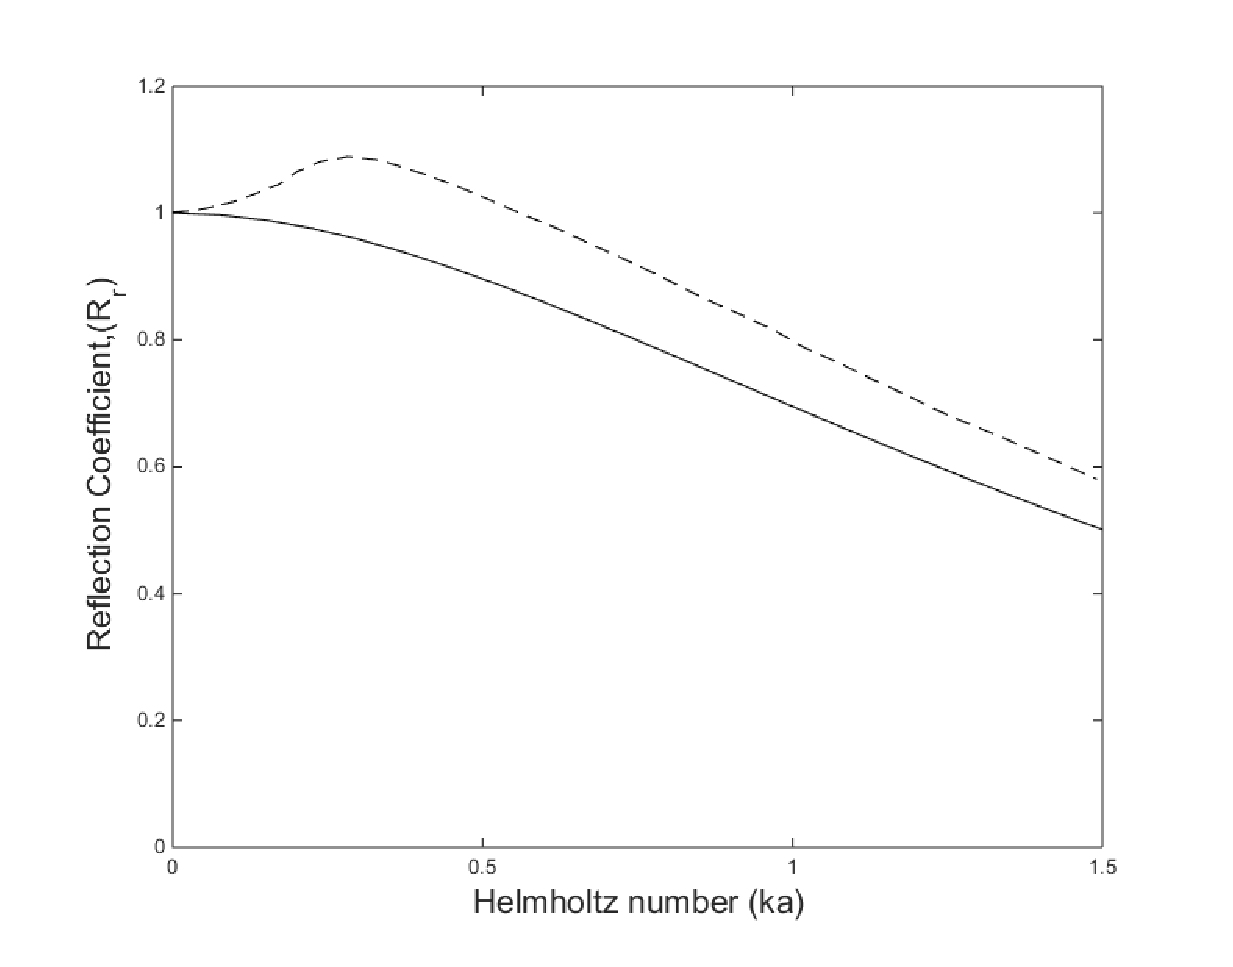
\includegraphics[width=.9\linewidth]{figuras/abs_r_comparacao.eps}
  \captionof{figure}{Resultados analíticos exatos para magnitude do coeficiente de reflexão $\|R\|$ ao final de um duto não flangeado. A linha contínua apresenta o resultado sem escoamento de \citeonline{levine1948radiation} e a linha tracejada apresenta o resultado com escoamento de \citeonline{munt1990acoustic}.}
  \label{fig:comp1}
\end{figure}

Como é mostrado na Figura \ref{fig:comp1}, a magnitude do coeficiente de reflexão $\|R\|$ aumenta consideravelmente mesmo na presença de um escoamento de baixo número de Mach. Além disso, pode-se perceber que, em algumas frequências, $\|R\|$ torna-se maior do que a unidade, implicando que a amplitude da onda refletida torna-se maior do que a da onda incidente. Este fenômeno ocorre, sobretudo, pela transferência de energia cinética rotacional do escoamento para o campo acústico. Essa transferência de energia cinética ocorre sobretudo pelo desprendimento periódico de vórtices na borda do duto.

\begin{figure}[ht!]
\centering
  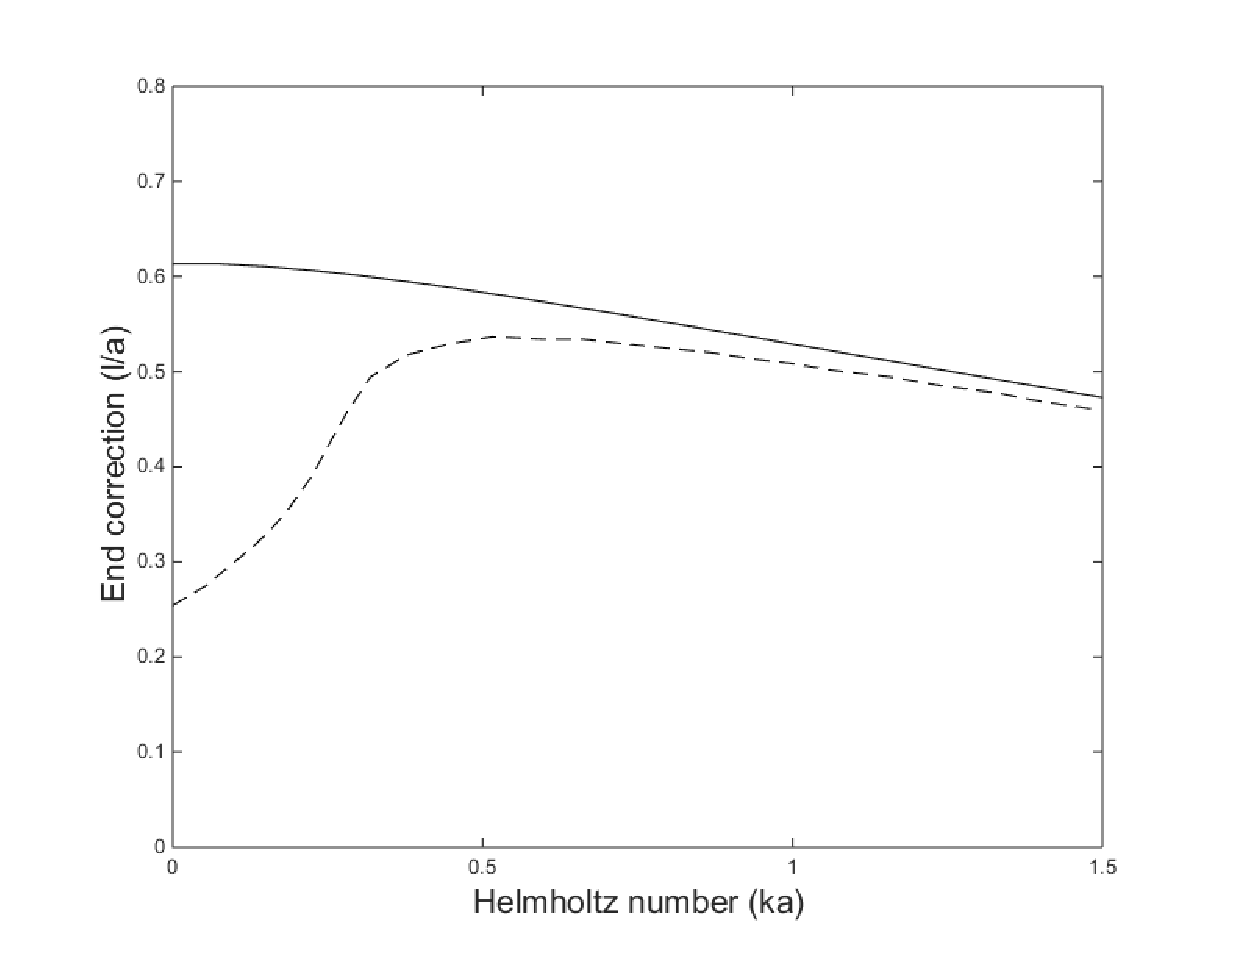
\includegraphics[width=.9\linewidth]{figuras/loa_comparacao.eps}
  \captionof{figure}{Resultados analíticos exatos para o coeficiente de correção da terminação normalizado pelo raio $l/a$ de um duto não flangeado. A linha contínua apresenta o resultado sem escoamento de \citeonline{levine1948radiation} e a linha tracejada apresenta o resultado com escoamento de \citeonline{munt1990acoustic}.}
  \label{fig:comp2}
\end{figure}

De acordo com a Figura \ref{fig:comp2}, a correção normalizada da terminação $l/a$ torna-se consideravelmente menor do que aquela obtida na ausência de escoamento, sobretudo para baixos números de $ka$. Em outras palavras, para baixas frequências e na presença de um escoamento a onda acústica é refletida em uma região mais próxima da abertura, em comparação à situação sem escoamento.


\begin{figure}[ht!]
\centering
  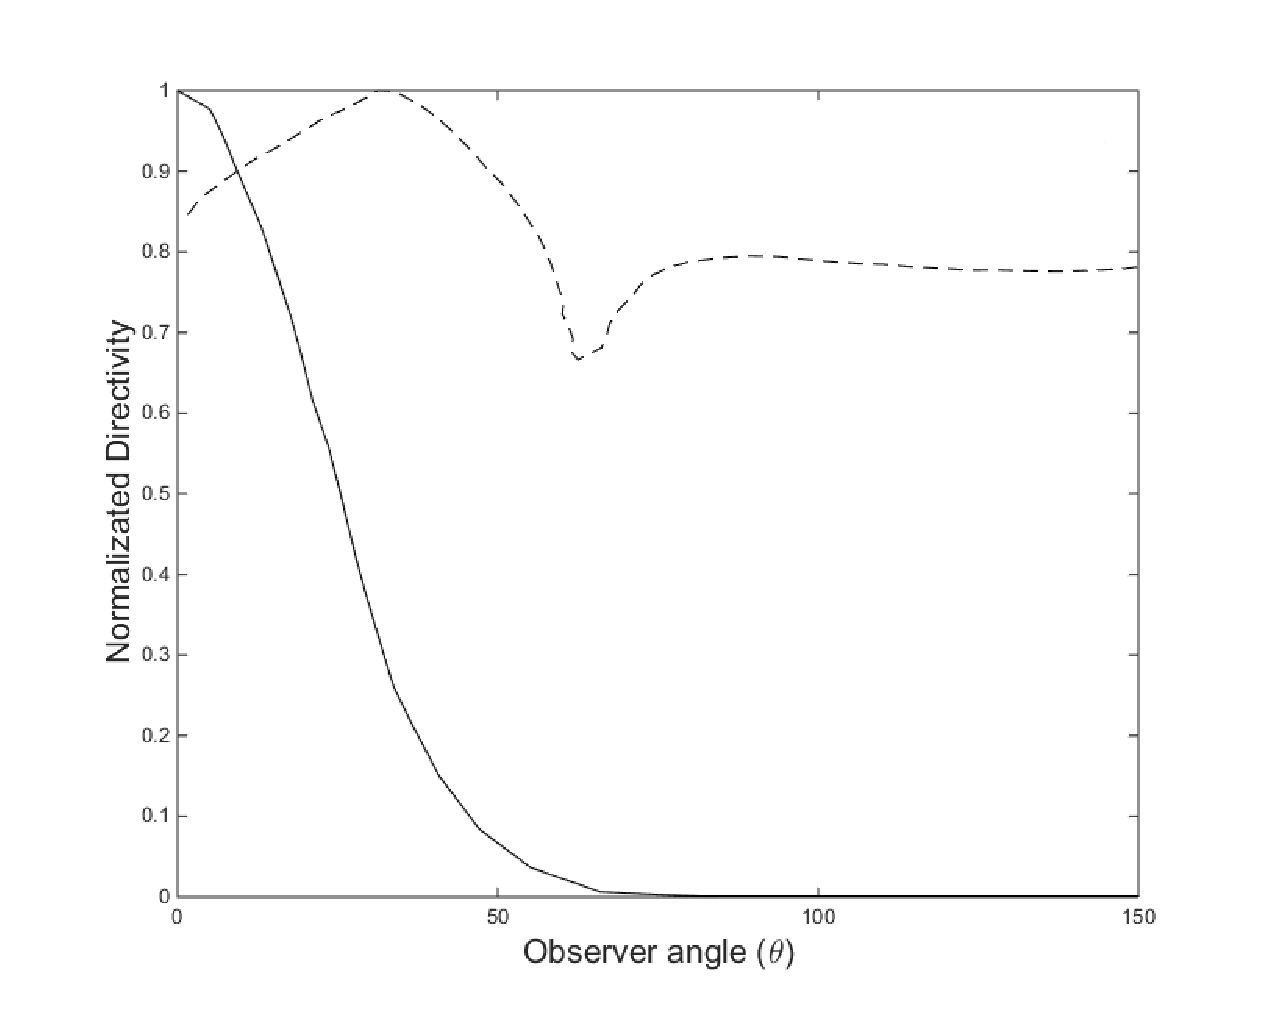
\includegraphics[width=.9\linewidth]{figuras/directivity_comparacao.eps}
  \captionof{figure}{Diretividade $G(f,\theta)$ para os valores de Mach = 0,134 e $ka$ = 4,58 para a curva tracejada de \citeonline{munt1977interaction} e $ka$ = 3,87 para a curva contínua de \citeonline{levine1948radiation}.}
  \label{fig:comp3}
\end{figure}

\newpage
De acordo com a Figura \ref{fig:comp3}, a diretividade $G(f,\theta)$ muda significativamente demonstrando maiores amplitudes em torno do ângulo de $45^{o}$ e há o fenômeno conhecido como zona de silêncio em torno do ângulo de $10^{o}$. Isto ocorre devido à refração de velocidade de fase. Mesmo as duas curvas tendo valores de $ka$ diferentes as diretividades normalizadas nos outros valores de $ka$ obedecem o mesmo padrão.

É importante ressaltar que modelos exatos para os parâmetros de radiação de dutos se limitam às condições geométricas simples. No entanto, observa-se na prática terminações cujas geometrias divergem significativamente daquela associadas a um duto não flangeado. Exemplos comuns destas geometrias são aquelas encontradas em difusores, chaminés, sistemas de exaustão, $nozzles$ e instrumentos musicais. A Figura \ref{fig:diferentes_dutos} ilustra casos mais realistas de terminação de dutos comumente encontrados na prática. Para estes casos, não existem modelos que considerem a influência do escoamento nas propriedades de radiação. Além disso, a análise numérica considerando os efeitos de escoamento não é trivial.

Considerando a problemática discutida acima, o objetivo principal deste trabalho é investigar, de forma numérica e experimental, o comportamento da magnitude dos coeficientes de reflexão $\|R\|$, correção da terminação $l/a$ e a diretividade $G(f,\theta)$ em dutos transportando escoamentos subsônicos (Mach $<$ 0,2), terminados com diferentes geometrias, incluindo cornetas cilíndricas e flanges de diferentes dimensões.

Tem-se como objetivos específicos:
\begin{itemize}
    \item modelagem numérica do duto não-flangeado sem escoamento;
    \item modelagem numérica do duto não-flangeado com escoamento;
    \item modelagem numérica do duto flangeado em cornetas cilíndricas com escoamento;
    \item validação experimental dos modelos numéricos;
    \item modelagem numérica do duto flangeado em cornetas cilíndricas com escoamento sugado.
\end{itemize}

\begin{figure}[ht!]
\centering
  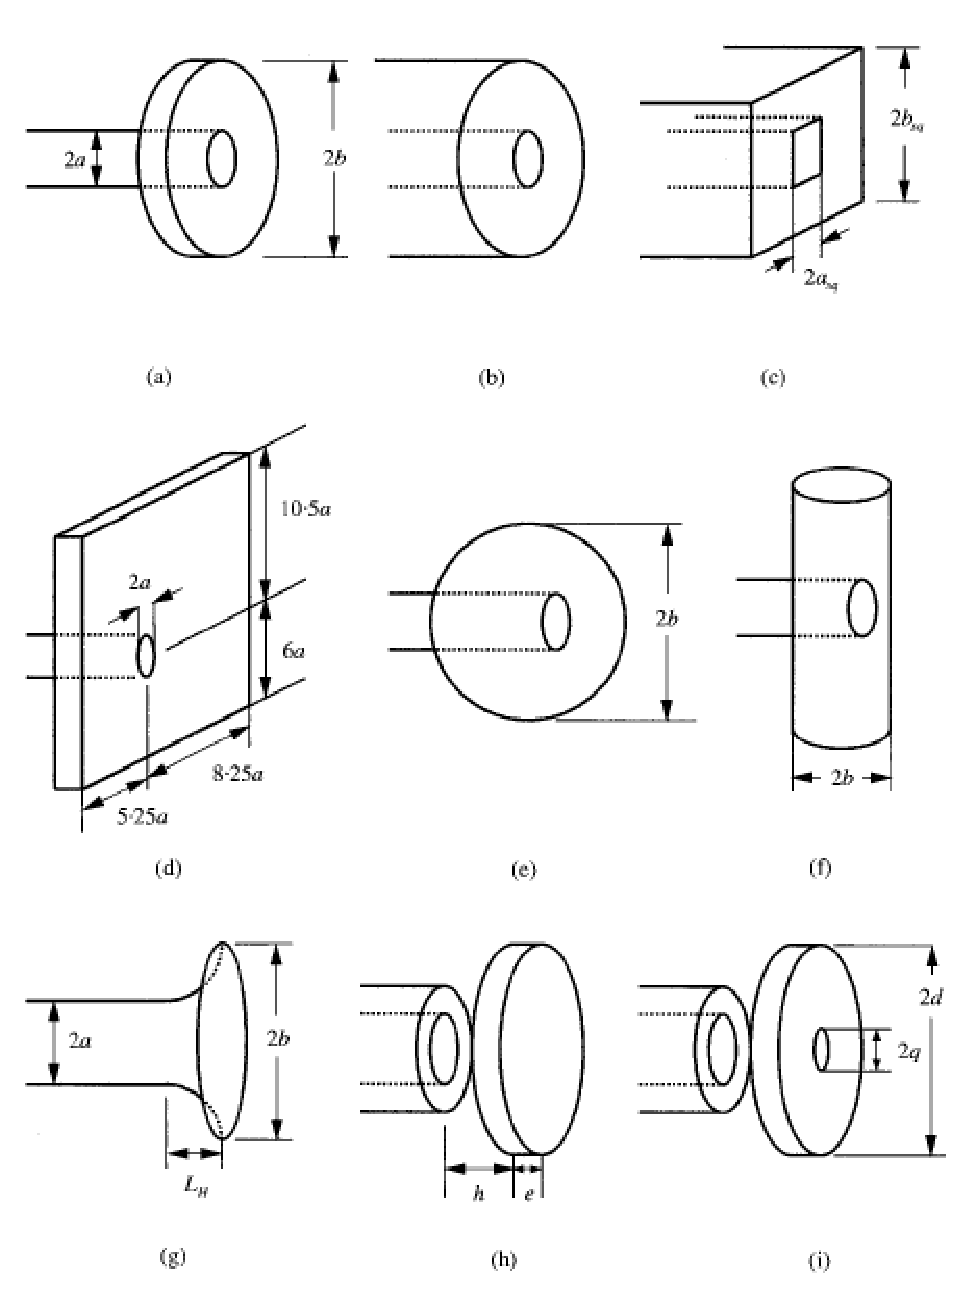
\includegraphics[width=.61\linewidth]{figuras/diferentes_dutos.eps}
  \\
  \text{Fonte: \cite{dalmont2001radiation}}
  \captionof{figure}{Exemplos de vários tipos de terminações: (a) flange circular; (b) flange circular com espessura do duto; (c) duto quadrado com flange de espessura quadrada; (d) flange normalizada; (e) flange esférica; (f) flange cilíndrica; (g) corneta; (h) disco não perfurado; (i) disco perfurado.}
  \label{fig:diferentes_dutos}
\end{figure}



\chapter{Revisão Bibliográfica}
\label{chapter:revisao}

Vários trabalhos foram feitos no contexto de irradiação normal de dutos, dentre os quais o mais canônico foi o trabalho de \citeonline{levine1948radiation}, que resolveu analiticamente o problema da radiação e da reflexão para terminação não-flangeada usando a técnica Wiener–Hopf. \citeonline{munt1977interaction} fez um trabalho similar desenvolvendo um modelo exato para a diretividade do som irradiado com escoamento subsônico. Posteriormente \citeonline{munt1990acoustic} complementou o modelo \\ adicionando o coeficiente de reflexão para números de Mach até 0,4. Usando teorias similares e considerando o escoamento como uniforme (\textit{plug}) o mesmo problema foi resolvido de maneira aproximada por  \citeonline{carrier1955sound} (usando o método de Prandtl-Glauert), \citeonline{mani1973refraction}, considerando o movimento transversal de ondas acústicas, e \citeonline{savkar1975radiation} considerando variações de temperatura. 

O modelo analítico \cite{munt1990acoustic} dos coeficientes de reflexão $\|R\|$ e correção de terminação $l/a$ foi validado experimentalmente por \citeonline{allam2006investigation}, utilizando um sistema de medição superdeterminado para a decomposição de onda. Mais recentemente esses resultados foram validados numericamente por \citeonline{da2009sound} e \citeonline{shi2013lattice}, usando método de lattice Boltzmann (LBM) com a condição de axissimetria proposta por \citeonline{halliday2001lattice}. 

Para modelos com diferentes terminações mas sem escoamento, \citeonline{dalmont2001radiation} determinaram o coeficiente de correção de terminação $l/a$ de forma experimental e numérica usando métodos de elementos de contorno e diferenças finitas, e \citeonline{selamet2001wave} determinaram os coeficientes de reflexão $\|R\|$ e correção de terminação $l/a$ usando método de elementos de contorno. Focando especificamente em flanges circulares, \citeonline{silva2012approximate} determinaram os coeficientes de reflexão $\|R\|$ e correção de terminação $l/a$ usando método de elementos de contorno.


Para a problemática de dutos com escoamentos e diferentes terminações, os métodos convencionais como elementos de contorno e diferenças finitas possuem várias limitações. Como alternativa de método, o LBM se mostra mais adequado quando se diz respeito a interações entre escoamentos e campos acústicos \cite{shi2013lattice}. Isto se deve à capacidade do método de resolver, numa mesma estrutura computacional, tanto o campo acústico quanto o campo fluido-dinâmico. Alguns trabalhos foram realizados para a aplicação do LBM em problemas acústicos e aeroacústicos. Um exemplo que possui aderência com o contexto desse trabalho é a validação do modelo de \citeonline{levine1948radiation} por \citeonline{da2006lattice}. \citeonline{crouse2006fundamental} demonstraram, através de quatro problemas canônicos em acústica, a aplicabilidade do LBM bem como a recuperação dos parâmetros macroscópicos da equação semi-compressível de Navier-Stokes. Um outro problema clássico de aerocústica para validação do LBM foi implementado por \citeonline{lew2010noise}, que investigaram o som em campo distante a partir de um jato turbulento subsônico. \citeonline{viggen2013acoustic} demonstrou a possibilidade de incluir fontes multipolos acústicos no LBM e os efeitos nos parâmetros macroscópicos relacionados a Navier-Stokes. Outro trabalho de \citeonline{viggen2014acoustic} foi propor diferentes equações de estado em LBM para poder simular efeitos de escoamentos de mais alta compressibilidade. 

Ainda no contexto do LBM, \citeonline{shi2013lattice} usaram o método para validar os resultados de diretividade de \citeonline{munt1977interaction}. Todavia o campo acústico processado era de campo próximo. A forma mais apropriada então para a captura de pressão é em campo distante. No entanto, isto demanda a construção de um domínio computacional relativamente grande para a captura da irradiação acústica em campo distante, o que, por sua vez, implica em alto custo computacional. Uma alternativa de solução para esse problema é a aplicação da superfície de Ffwocs Willians-Hawkings (FW-H) proposta por \citeonline{lockard2000efficient}. Um exemplo de aplicação dessa formulação junto com o LBM é o trabalho de \citeonline{da2015assessment}, que constituiu o campo distante de um ruído oriundo da instalação de uma placa próximo a um jato.

Outra problemática relativa à modelagem numérica usando LBM é a implementação de uma condição anecóica. Essa condição consiste em, além de absorver o som gerado pelos processos aerodinâmicos, absorver também o escoamento e a vorticidade gerada. Algumas opções de condições anecóicas são a condição ABC de \citeonline{kam2006non} que se baseia numa região de amortecimento redirecionando os valores de densidade e velocidade das partículas para um valor alvo, e a condição de \citeonline{najafi2012absorbing} que implementa uma formulação de \textit{Perfectly Matched Layer} (PML) para LBM.

\chapter{Metodologia}
\label{chapter:metodologia}

Além da revisão bibliográfica apresentada, a condução do presente trabalho dar-se-á pelas seguintes etapas:
\begin{enumerate}
    \item Modelagem numérica do duto não-flangeado sem escoamento. Para tal fim é preciso definir o domínio fluido-dinâmico de tal forma que o campo acústico possa ser corretamente definido sem muitas distorções, também é preciso definir o duto com paredes rígidas com condição \textit{bounce back} e sua forma de excitação sonora e, por fim, definição de condições de contorno anecóicas para o campo acústico não sofrer contaminações oriundas das reflexões. Para tanto, serão feitos os seguintes procedimentos:
        \begin{enumerate}
            \item implementação da condição anecóica em 3 dimensões proposta por Najafi-Yazdi e Mongeau \cite{najafi2012absorbing} no \textit{software} Palabos;
            \item validação da condição anecóica no \textit{software} Palabos determinando $\|R\|$ e $l/a$ num duto simples;
            \item validação do modelo comparando com os resultados de Levine e Schwinger \cite{levine1948radiation} através dos parâmetros $\|R\|$ e $l/a$;
            \item implementação da superfície de FW-H no software Palabos;
            \item validação da superfície de FW-H para diretividade $G(f,\theta)$ com os resultados de Levine e Schwinger \cite{levine1948radiation}.
        \end{enumerate}
        
    \item Modelagem numérica do duto não-flangeado com escoamento. A partir do modelo sem escoamento, será inserido um termo fonte baseado na formulação de \citeonline{kam2006non} que criará um escoamento no interior do duto. Dado esse contexto é preciso realizar as seguintes etapas:
        \begin{enumerate}
            \item determinação e validação com os resultados de Munt \cite{munt1990acoustic} de $\|R\|$ e $l/a$ para números de Mach 0,05, 0,1 e 0,15;
            \item determinação de $G(f,\theta)$ e validação com os resultados de Munt \cite{munt1990acoustic} e Shi Yong et al. \cite{shi2013lattice}.
        \end{enumerate}
        
    \item Modelagem numérica do duto com cornetas cilíndricas com escoamento. Para a definição de cornetas em LBM é preciso definir uma condição de paredes curvas não-alinhadas como por exemplo a de \citeonline{bouzidi2001momentum}. Para tal fim deverá ser feito:
        \begin{enumerate}
            \item simulação para cornetas $2r$ e $4r$, tal que $r$ é o raio de curvatura da corneta, determinando $\|R\|$, $l/a$ e $G(f,\theta)$ segundo o trabalho \cite{da2009sound}.
        \end{enumerate}
    
    \item Validação experimental dos modelos numéricos. Essa etapa será realizada no rig de jato do laboratório de vibrações e acústica e será baseada no experimento de \citeonline{allam2006investigation} de acordo com a configuração mostrada na Figura \ref{fig:duto_abom}. Dado o exposto, para essa etapa os seguintes procedimentos deverão ser feitos:
    \begin{enumerate}
            \item projeto e implantação do \textit{rig} de jato de acordo com o estudo \cite{allam2006investigation};
            \item projeto e confecção das cornetas cilíndricas para terminação do duto;
            \item determinação de $\|R\|$ e $l/a$ com os microfones internos; 
            \item determinação de $G(f,\theta)$ com o \textit{array} de microfones externos. 
        \end{enumerate}
    \begin{figure}[ht!]
    \centering
      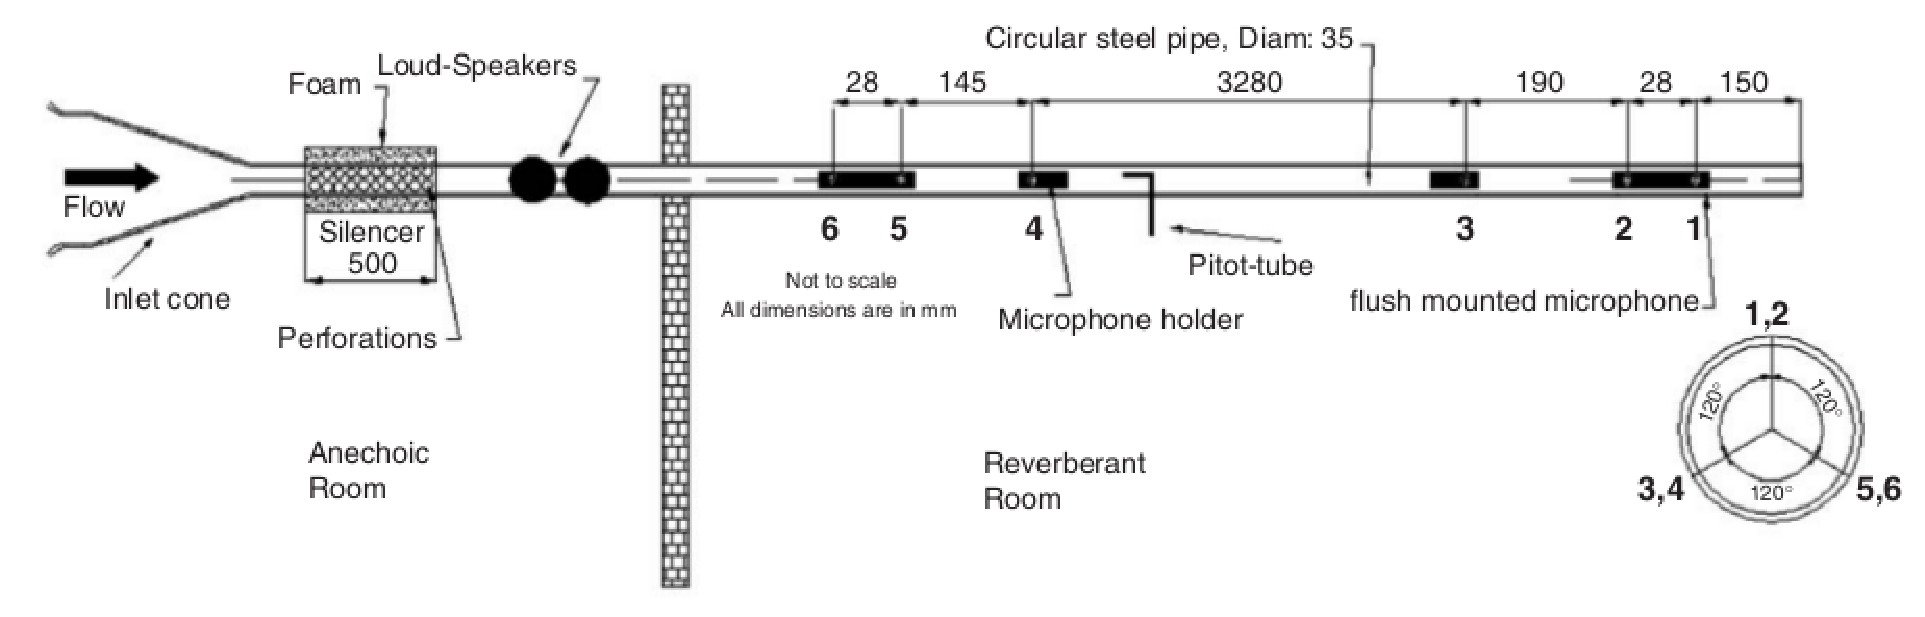
\includegraphics[width=.95\linewidth]{figuras/duto_abom.eps}
      \\
      \text{Fonte: \cite{allam2006investigation}}
      \captionof{figure}{Esquema de configuração do duto.}
      \label{fig:duto_abom}
    \end{figure}
    
    \item Modelagem numérica do duto flangeado em cornetas cilíndricas com escoamento sugado. Dado o modelo numérico validado, pode-se agora redimensionar os parâmetros alvos de pressão e velocidade da condição de \citeonline{kam2006non} de tal forma que o escoamento mude de sentido. Esse fato possibilitará a realização da seguinte etapa:
        \begin{enumerate}
            \item determinação de $\|R\|$, $l/a$ e $G(f,\theta)$;
        \end{enumerate}
    \item redação da dissertação.
\end{enumerate}
 

\chapter{Resultados Preliminares}
\label{chapter:resultados}

No que diz respeito aos resultados preliminares, foi implementado e simulado o modelo numérico descrito no estudo de \citeonline{shi2013lattice}. Basicamente é um duto com a terminação aberta não-flangeada que teve os modos excitados junto com escoamento. A Figura \ref{fig:duto_1} mostra os resultados comparados para $\|R\|$ e correção da terminação $l/a$. Percebe-se que os resultados apresentam boa convergência com os resultados da literatura.

\begin{figure}[h]
	\centering
	 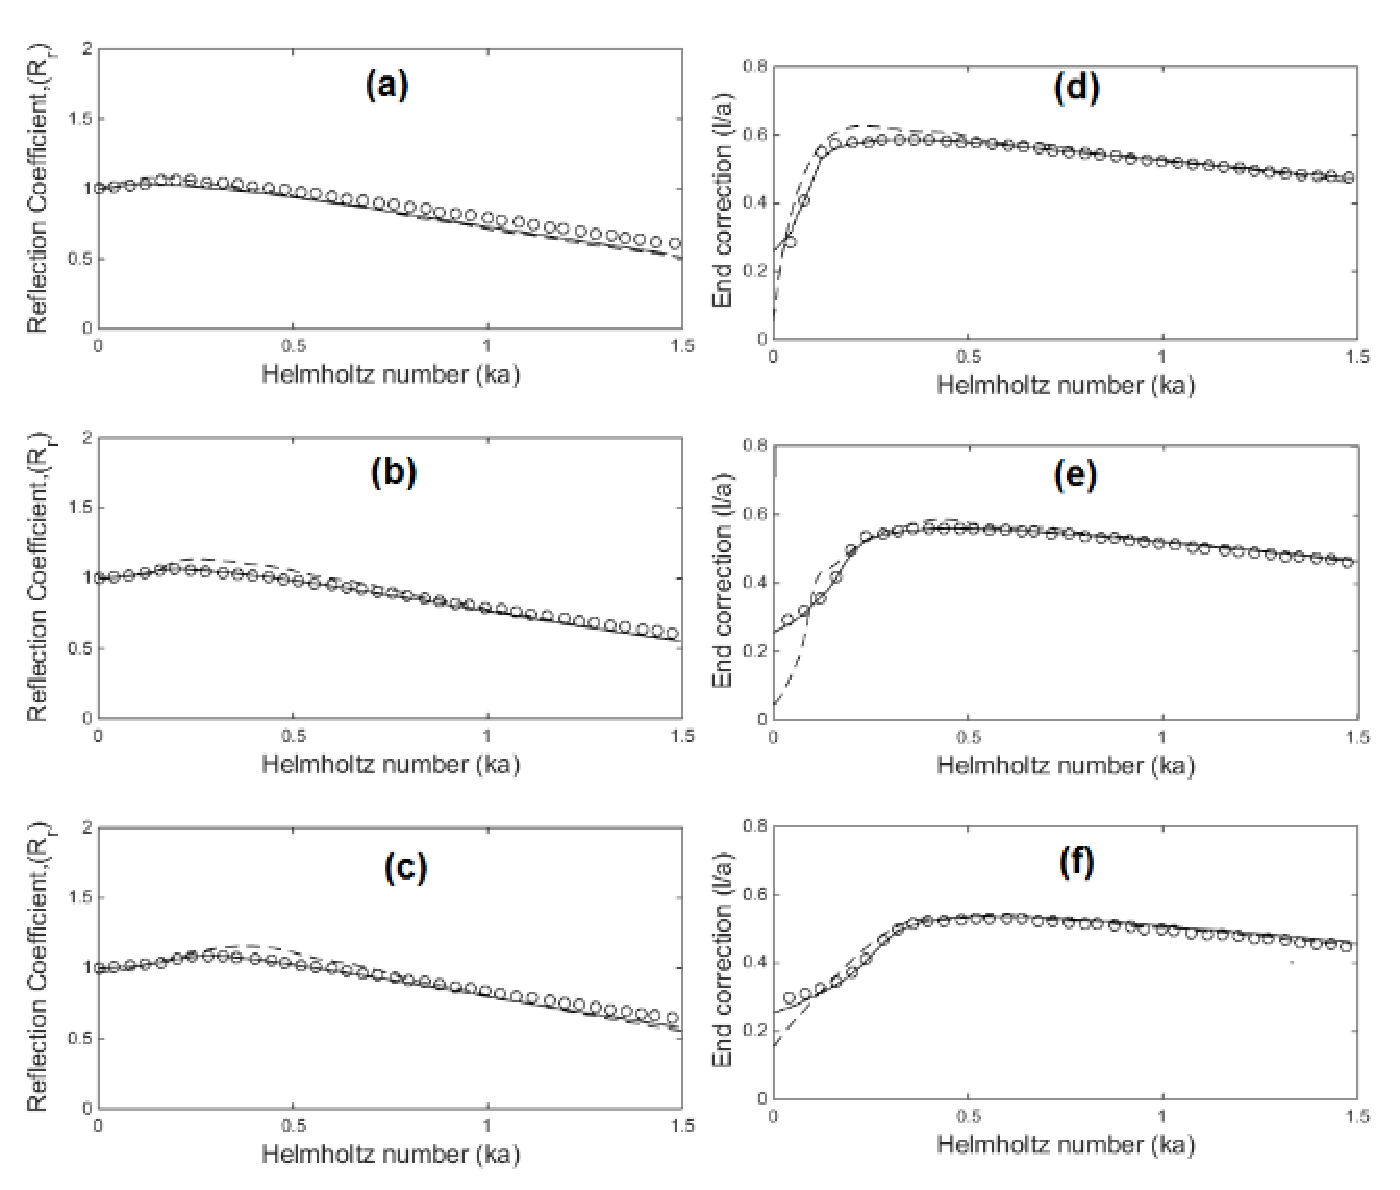
\includegraphics[width=9.5cm, height=9.5cm]{figuras/duto_1.eps}
	\caption{Comparação entre resultados analítico de \citeonline{munt1990acoustic} (linha sólida), resultados de \citeonline{da2009sound} (círculo vazio) e a presente modelagem numérica (linha traçada) para magnitude de $\|R\|$ com números de Mach 0,05 (a), 0,1 (b) e 0,15 (c) e correção da terminação $l/a$ normalizado pelo raio do duto com números de Mach 0,05 (d), 0,1 (e) e 0,15(f).}
	\label{fig:duto_1}
\end{figure}

\newpage
As Figuras \ref{fig:duto_2_1}, \ref{fig:duto_2_2}, \ref{fig:duto_2_3} e \ref{fig:duto_2_4} mostram os resultados comparados com estudos anteriores para a diretividade $G(f,\theta)$. É perceptível que os resultados da presente modelagem numérica com a superfície de FW-H estão com uma boa convergência.

\begin{figure}[ht!]
	\centering
	 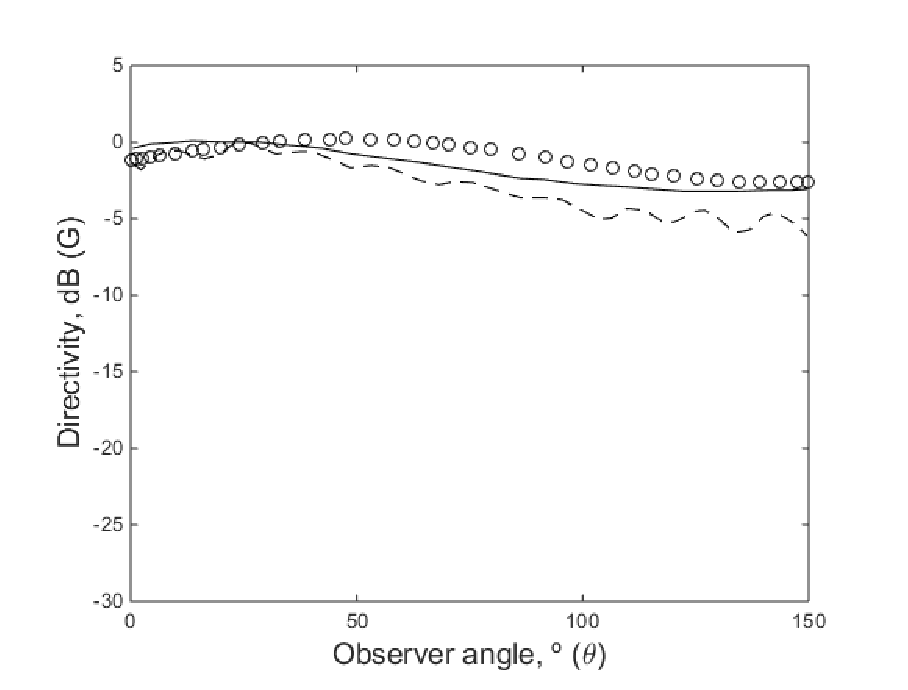
\includegraphics[width=10cm, height=5cm]{figuras/ka_074_0036.eps}
	\caption{Comparação entre resultados analíticos de \citeonline{munt1990acoustic} (linha sólida), numéricos de \citeonline{shi2013lattice} (linha traçada) e a presente modelagem numérica (círculos vazios) para diretividade $G(f,\theta)$, em dB, para o caso ka = 0,74 e Mach = 0,036.}
	\label{fig:duto_2_1}
\end{figure}

\begin{figure}[ht!]
	\centering
	 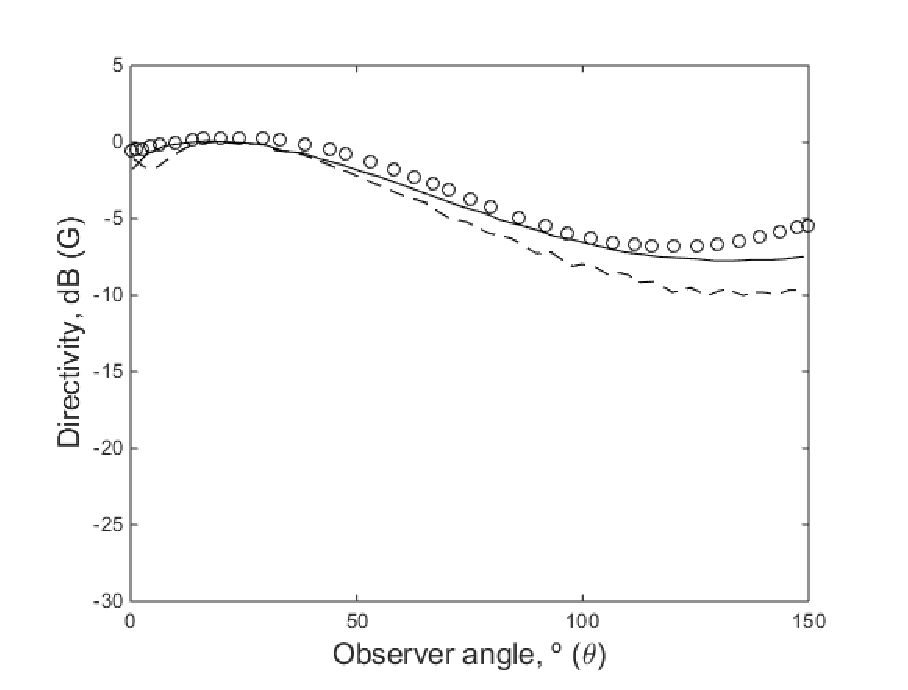
\includegraphics[width=10cm, height=5cm]{figuras/ka_148_0036.eps}
	\caption{Comparação entre resultados analíticos de \citeonline{munt1990acoustic} (linha sólida), numéricos de \citeonline{shi2013lattice} (linha traçada) e a presente modelagem numérica (círculos vazios) para diretividade $G(f,\theta)$, em dB, para o caso ka = 1,48 e Mach = 0,036.}
	\label{fig:duto_2_2}
\end{figure}

\begin{figure}[ht!]
	\centering
	 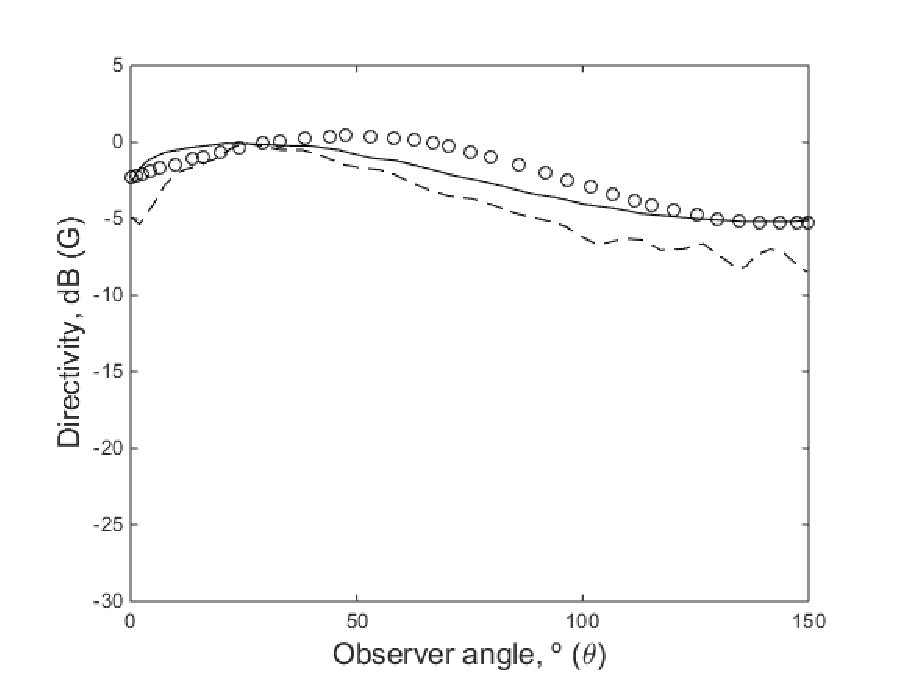
\includegraphics[width=10cm, height=5cm]{figuras/ka_074_015.eps}
	\caption{Comparação entre resultados analíticos de \citeonline{munt1990acoustic} (linha sólida), numéricos de \citeonline{shi2013lattice} (linha traçada) e a presente modelagem numérica (círculos vazios) para diretividade $G(f,\theta)$, em dB, para o caso ka = 0,74 e Mach = 0,15.}
	\label{fig:duto_2_3}
\end{figure}

\begin{figure}[ht!]
	\centering
	 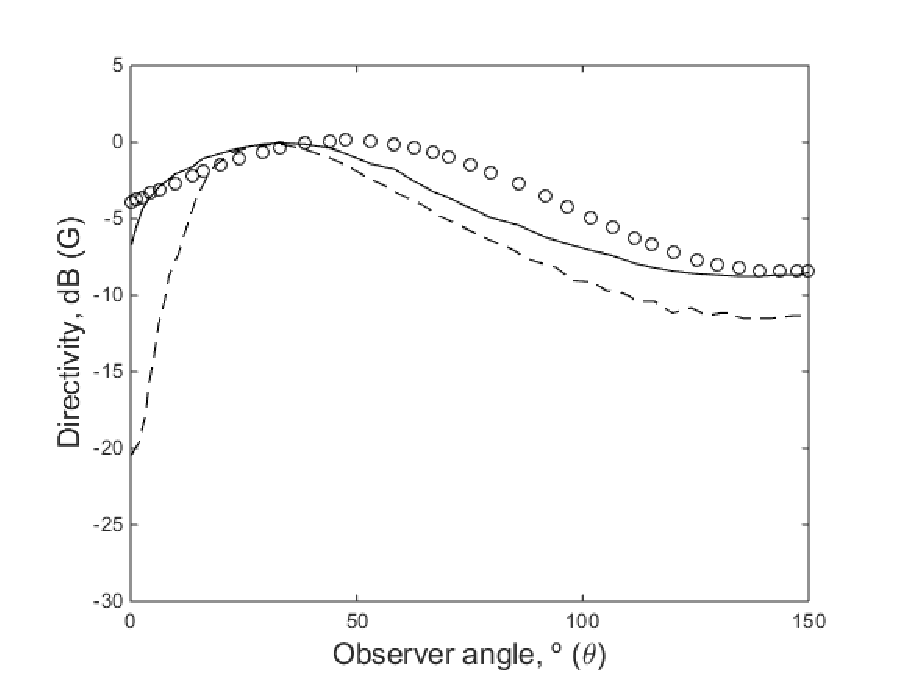
\includegraphics[width=10cm, height=5cm]{figuras/ka_148_015.eps}
	\caption{Comparação entre resultados analíticos de \citeonline{munt1990acoustic} (linha sólida), numéricos de \citeonline{shi2013lattice} (linha traçada) e a presente modelagem numérica (círculos vazios) para diretividade $G(f,\theta)$, em dB, para o caso ka = 1,48 e Mach = 0,15.}
	\label{fig:duto_2_4}
\end{figure}

Em vista das simulações abordadas, pode-se verificar que a implementação dos modelos em LBM estão coerentes e gerando boas concordâncias com estudos anteriores, todavia ainda pode-se melhorar os resultados com o uso da superfície de FW-H aplicando-a num contexto de modelagem numérica em 3 dimensões.

\chapter{Cronograma}
\label{chapter:cronograma}
% Please add the following required packages to your document preamble:
\begin{table}[ht!]
\centering
\caption{Cronograma de Atividades}
\label{my-label}
\begin{tabular}{|c|l|l|l|l|l|l|l|l|l|l|l|l|l|}
\hline
\multicolumn{1}{|l|}{Atividades} & \multicolumn{7}{c|}{2016}                                                                                                                                                    & \multicolumn{6}{c|}{2017}                                                            \\ \cline{2-14} 
\multicolumn{1}{|l|}{}                            & 6                      & 7                      & 8                      & 9                      & 10                     & 11                     & 12                     & 1                      & 2                      & 3                      & 4 & 5 & 6 \\ \hline
1                                                 & \multicolumn{1}{c|}{x} & \multicolumn{1}{c|}{x} & \multicolumn{1}{c|}{x} & \multicolumn{1}{c|}{x} & \multicolumn{1}{c|}{x} & \multicolumn{1}{c|}{x} & \multicolumn{1}{c|}{x} & \multicolumn{1}{c|}{x} & \multicolumn{1}{c|}{x} & \multicolumn{1}{c|}{x} &   &   &   \\ \hline
2.a                                               & x                      & x                      &                        &                        &                        &                        &                        &                        &                        &                        &   &   &   \\ \hline
2.b                                               &                        & x                      &                        &                        &                        &                        &                        &                        &                        &                        &   &   &   \\ \hline
2.c                                               &                        & x                      &                        &                        &                        &                        &                        &                        &                        &                        &   &   &   \\ \hline
2.d                                               &                        &                        & x                      &                        &                        &                        &                        &                        &                        &                        &   &   &   \\ \hline
2.e                                               &                        &                        & x                      &                        &                        &                        &                        &                        &                        &                        &   &   &   \\ \hline
3.a                                               &                        &                        &                        & x                      &                        &                        &                        &                        &                        &                        &   &   &   \\ \hline
3.b                                               &                        &                        &                        & x                      &                        &                        &                        &                        &                        &                        &   &   &   \\ \hline
4.a                                               &                        &                        &                        &                        & x                      &                        &                        &                        &                        &                        &   &   &   \\ \hline
5.a                                               &                        &                        &                        &                        & x                      & x                      &                        &                        &                        &                        &   &   &   \\ \hline
5.b                                               &                        &                        &                        &                        & x                      & x                      & x                      &                        &                        &                        &   &   &   \\ \hline
5.c                                               &                        &                        &                        &                        &                        &                        & x                      & x                      &                        &                        &   &   &   \\ \hline
5.d                                               &                        &                        &                        &                        &                        &                        & x                      & x                      & x                      &                        &   &   &   \\ \hline
6.a                                               &                        &                        &                        &                        &                        &                        &                        &                        & x                      & x                      &   &   &   \\ \hline
7                                                 &                        &                        &                        &                        &                        &                        &                        & x                       & x                       &  x                      & x & x & x \\ \hline
\end{tabular}
\end{table} 
%\chapter{Conceituação Teórica}

%\chapter{Metodologia}

%\chapter{Etapas do trabalho}

%\chapter{Cronograma}
Neste tópico será abordado a duração de cada uma das etapas de trabalho como pode ser visto na \figura{fig_cronograma}. Desta forma será possível uma melhor organização do mesmo.

\begin{figure}[H]
    \centering
    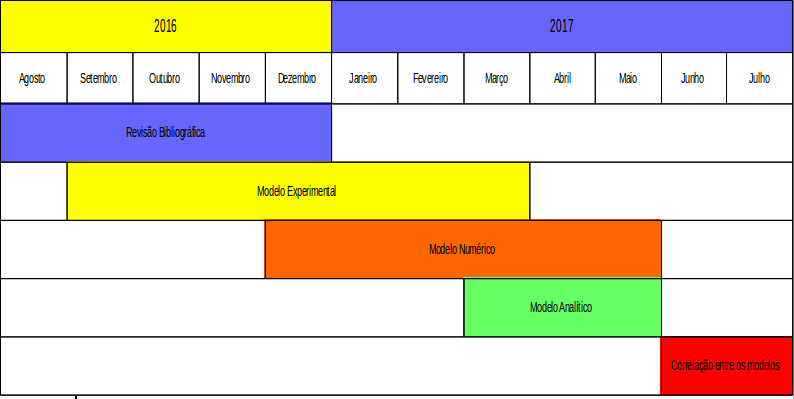
\includegraphics[width=10cm]{figuras/cronograma.png}
    \caption{Elaborado pelo autor.}
    \label{fig_cronograma}
\end{figure}


%%%%%%%%%%%%%%%%%%%%%%%%%%%%%%%%%%%%%%%%%%%%%%%%%%%%%%%%%%%%%%%%%%%%%%%%%


\bibliographystyle{ufscThesis/ufsc-alf}
\bibliography{bibliografia}
%%%%%%%%%%%%%%%%%%%%%	REFERÊNCIAS    %%%%%%%%%%%%%%%%%%%%%%%%%%%%%%%%%%%

%--------------------------------------------------------
% Elementos pós-textuais
%\apendice
%\chapter{Exemplificando um Apêndice}
%Texto do Apêndice aqui. 

%\anexo
%\chapter{Exemplificando um Anexo}
%Texto do anexo aqui.
\end{document}
